\section{Evaluating the performance of the proposed method}
\label{sec:rul_eval}

In this section we evaluate the performance of the proposed method. The architecture of the \gls{mlp} to be used here was presented in Section \ref{sec:method} Table \ref{table:proposed_nn} and will be used throughout this section.  The \gls{mlp} was trained $10$ times for$200$ epochs each and tested in each subset of the \gls{cmaps} dataset.

For the first experiment the combinations of window size $n_w$, window stride $n_s$ and early \gls{rul} $R_e$ presented in Table \ref{table:data_params_de} were tested obtaining the results shown in Table \ref{table:results_ann_de}.

\begin{table}[!htb]
\centering
\begin{tabular}{l l l l l}
	\hline
	 Dataset & Window Size $n_w$ & Window Stride $n_s$ & Early RUL $R_e$\\
  	\hline
  	FD001 & 30 & 2 & 120\\
  	FD002 & 20 & 2 & 120\\
  	FD003 & 30 & 2 & 120\\
  	FD004 & 18 & 2 & 120\\
  	\hline
\end{tabular}
\caption{Data-related parameters for each subset as obtained by \gls{de}.}
\label{table:data_params_de}
\end{table}  

\begin{table}[!htb]
\centering

\begin{tabular}{l | r r r r | r r r r}
	\hline	
	& \multicolumn{4}{| c}{RMSE} & \multicolumn{4}{| c}{RHS} \\
	Data Subset & Min. & Max. & Avg. & STD & Min. & Max. & Avg. & STD\\
  	\hline
  	FD001 & 15.01 & 16.46 & 15.43 & 0.42 & 3.50 & 4.24 & 3.80 & 0.24\\
  	FD002 & 29.94 & 31.12 & 30.51 & 0.49 & 48.81 & 86.14 & 64.38 & 13.18\\
  	FD003 & 15.00 & 16.39 & 15.45 & 0.47 & 3.24 & 4.57 & 3.80 & 0.45\\
  	FD004 & 33.42 & 36.78 & 34.52 & 0.99 & 54.19 & 72.68 & 62.02 & 6.68\\
  	\hline
\end{tabular}

\caption{Scores for each dataset using the data-related parameters obtained by \gls{de}.}
\label{table:results_ann_de}
\end{table}

Next, the possibility of using a single set of data-related parameters for all the subsets is explored. For this experiment the window size $n_w$ is fixed for all of the four datasets, given that the maximum allowable window size for all datasets is $18$, $n_w = 18$ will be used as window size throughout the four subsets. Details of the data-related chosen parameters are presented in Table \ref{table:data_params_1}, the results obtained are shown in Table \ref{table:results_ann_1}. 

\begin{table}[!htb]
\centering
\begin{tabular}{l l l l l}
	\hline
	 Dataset & Window Size $n_w$ & Window Stride $n_s$ & Early RUL $R_e$\\
  	\hline
  	FD001 & 25 & 2 & 95\\
  	FD002 & 15 & 2 & 95\\
  	FD003 & 25 & 2 & 95\\
  	FD004 & 15 & 2 & 95\\
  	\hline
\end{tabular}
\caption{Rectified data-related parameters for each subset.}
\label{table:data_params_1}
\end{table}  

\begin{comment}
\begin{table}[!htb]
\centering
\begin{tabular}{l r r | r r | r r | r r}
	\hline	
	& \multicolumn{2}{c}{Min.} & \multicolumn{2}{c}{Max.}  & \multicolumn{2}{c}{Avg.}  & \multicolumn{2}{c}{STD} \\
	Data Subset & RMSE & RHS & RMSE & RHS & RMSE & RHS & RMSE & RHS\\
  	\hline
  	FD001 & 10.50 & 158.04 & 12.57 & 187.81 & 10.94 & 167.73 & 0.60 & 9.90\\
  	FD002 & 16.05 & 1551.98 & 18.70 & 2015.90 & 16.86 & 1756.61 & 0.86 & 166.03\\
  	FD003 & 10.83 & 142.31 & 17.93 & 343.98 & 12.09 & 174.46 & 2.19 & 61.23\\
  	FD004 & 22.36 & 6157.60 & 23.78 & 9221.86 & 22.82 & 7225.61 & 0.50 & 909.09\\
  	\hline
\end{tabular}
\caption{Scores for each dataset using the rectified data-related parameters.}
\label{table:results_ann_1}
\end{table}
\end{comment}

\begin{table}[!htb]
\centering
\begin{tabular}{l | r r r r | r r r r}
	\hline	
	& \multicolumn{4}{| c}{RMSE} & \multicolumn{4}{| c}{RHS} \\
	Data Subset & Min. & Max. & Avg. & STD & Min. & Max. & Avg. & STD\\
  	\hline
  	FD001 & 10.50 & 12.57 & 10.94 & 0.60 & 158.04 & 187.81 & 167.73 & 9.90\\
  	FD002 & 16.05 & 18.70 & 16.86 & 0.86 & 1551.98 & 2015.90 & 1756.61 & 166.03\\
  	FD003 & 10.83 & 17.93 & 12.09 & 2.19 & 142.31 & 343.98 & 174.46 & 61.23\\
  	FD004 & 22.36 & 23.78 & 22.82 & 0.50 & 6157.60 & 9221.86 & 7225.61 & 909.09\\
  	\hline
\end{tabular}
\caption{Scores for each dataset using the rectified data-related parameters.}
\label{table:results_ann_1}
\end{table}

\pagebreak

The above results show that slight variations to the time window barely hurts the performance of the regressor. Going one step further, trying a single set of data-related parameters is explored in the following experiment. The values used for the data related parameters are displayed in Table \ref{table:data_params_2}, the results obtained by the regressor using such parameters are shown in Table \ref{table:results_ann_2}.

\begin{table}[!htb]
\centering
\begin{tabular}{l l l l l}
	\hline
	 Dataset & Window Size $n_w$ & Window Stride $n_s$ & Early RUL $R_e$\\
  	\hline
  	All & 15 & 2 & 95\\
  	\hline
\end{tabular}
\caption{Single set of data-related parameters for all subsets.}
\label{table:data_params_2}
\end{table}  

\begin{table}[!htb]
\centering
\begin{tabular}{l | r r r r | r r r r}
	\hline	
	& \multicolumn{4}{| c}{RMSE} & \multicolumn{4}{| c}{RHS} \\
	Data Subset & Min. & Max. & Avg. & STD & Min. & Max. & Avg. & STD\\
  	\hline
  	FD001 & 12.26 & 13.83 & 12.95 & 0.52 & 237.42 & 352.26 & 290.70 & 38.52\\
  	FD002 & 16.15 & 18.18 & 16.85 & 0.69 & 1522.32 & 1910.06 & 1732.36 & 152.05\\
  	FD003 & 11.20 & 13.57 & 12.14 & 0.63 & 165.81 & 227.31 & 200.01 & 16.74\\
  	FD004 & 20.91 & 22.72 & 21.92 & 0.72 & 5497.36 & 7210.30 & 6126.21 & 570.17\\
  	\hline
\end{tabular}
\caption{Scores for each dataset using the single set of data-related parameters.}
\label{table:results_ann_2}
\end{table}

\pagebreak

As can be observed, most of the results remain unchanged except for subset FD001 where performance was decreased, nevertheless the use of a single set of data-related parameters is still promising and worth of more exploration. Figures \ref{fig:scores_rmse} and \ref{fig:scores_rhs} show a comparison of how the scores are affected for each dataset by changing the data-related parameters to make use of 4, 2 and 1 set of them.

\begin{figure}[!htb]
\centering
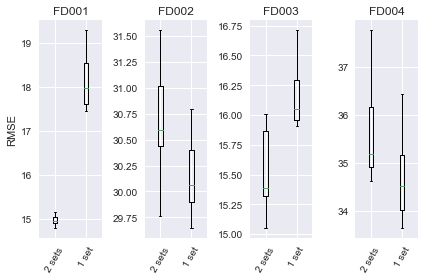
\includegraphics[width=0.5\textwidth]{img/rmse_comparisson.png}
\caption{Comparison of \gls{rmse} results for different sets of data-related parameters.}
\label{fig:scores_rmse}
\end{figure}

\begin{figure}[!htb]
\centering
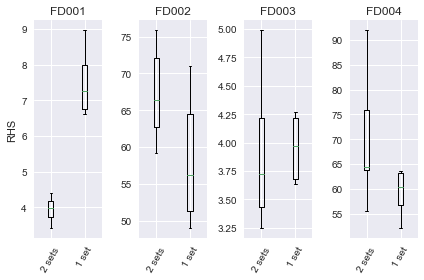
\includegraphics[width=0.5\textwidth]{img/rhs_comparisson.png}
\caption{Comparison of \gls{rhs} results for different sets of data-related parameters.}
\label{fig:scores_rhs}
\end{figure}